\section{EELS analyses of TMDs nanostructures}
\label{sec:tmdeels}

In this work we apply our machine learning method to the study
of the low-loss EELS region for a specific type of WS$_2$ nanostructures known
as nanoflowers.
%
WS$_2$ is a transition metal dichalcogenide (TMD) material, which in turn
belongs to a class of materials known as two-dimensional, van der Waals, or simply layered materials.
%
These materials are
characterised by the remarkable property of being fully functional down to a single atomic layer.
%
In order to make the present study self-contained and accessible to a wider audience,
in this section we review the basic concepts underlying the EELS
method and discuss some of its recent applications to the study of TMDs nanostructures with emphasis
on WS$_2$.

\subsection{EELS and its ZLP in a nutshell}
\label{sec:tmd}

Electron energy loss spectroscopy is a TEM-based method
whereby an electron-transparent sample is illuminated by a 
beam of energetic electrons.
%
Subsequent to the crossing of
the specimen, the scattered electron beam is focused by a magnetic prism
towards a spectrometer where the distribution of electron energy losses $\Delta E$ is recorded.
%
A schematic illustration of a typical EELS setup shown in the left panel of Fig.~\ref{fig:EELS}.
%
EEL spectra can be recorded either in the Scanning Transmission Electron Microscopy (STEM) mode
or in the conventional TEM setup.
%
Thanks to recent progress in TEM instrumentation and data acquisition, state-of-the-art EELS analyses benefit from
a highly competitive energy (spectral) resolution combined with an unparalleled spatial resolution.

%%%%%%%%%%%%%%%%%%%%%%%%%%%%%%%%%%%%%%%%%%%%%%%
\begin{figure}[t]
    \centering
    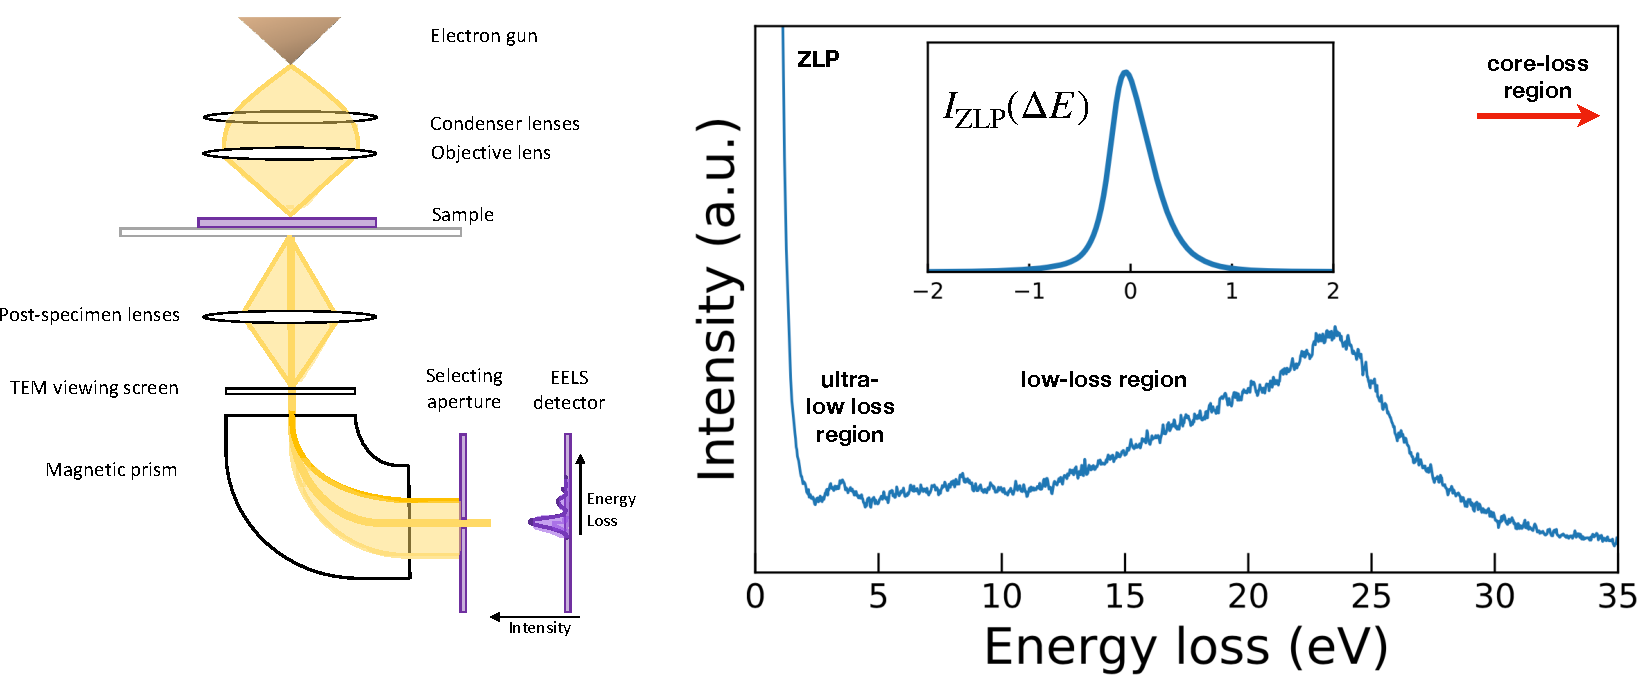
\includegraphics[width=0.9\textwidth]{plots/EELS.pdf}
    \caption{Left: in STEM-EELS, a magnetic
      prism is used to deflect the electron beam after crossing the sample
      so that the distribution of their energy losses $\Delta E$ can be recorded.
      %
      Right: a representative spectrum for $\Delta E \le 35$ eV acquired 
      on a WS$_2$ nanoflower~\cite{SabryaWS2} with
      the inset displaying the corresponding ZLP.
      }
    \label{fig:EELS}
\end{figure}
%%%%%%%%%%%%%%%%%%%%%%%%%%%%%%%%%%%%%%%%%%%%%%%%5

EELS spectra can be divided into three main regions.
%
The first is the zero-loss region, which is centered around $\Delta E=0$
and contains the contributions from both elastic scatterings
as well as those from electrons that have not interacted with the
sample.
%
This region is characterised by the strong and narrow zero-loss peak (ZLP)
which is much larger than the contribution
from inelastic scatterings.
%
The second region is the low-loss region, defined for energy losses
$\Delta E \lsim 50$ eV, which contains information
about several important features such as plasmons, excitons, phonons and
intra-band transitions.
%
Of particular relevance in this context is the ultra-low loss region, characterised by $\Delta E \simeq$ few eV.
Here, the contributions of the ZLP and those from the inelastic interactions
with the sample are of the same order of magnitude.
%
The regime for $\Delta E \gsim 50$ eV is the core-loss region,
which provides compositional information
on the materials that constitute the sample.
 
The right panel of Fig.~\ref{fig:EELS} displays
a representative EELS spectrum in the region $\Delta E \le 35$ eV, recorded
in one of the WS$_2$ nanostructures presented in~\cite{SabryaWS2}
and which will be further discussed later onwards.
%
The inset displays the ZLP, illustrating how nearby $\Delta E\simeq 0$
its magnitude is larger than the contribution from the inelastic scatterings
off the sample by several
orders of magnitude.
%
Carefully disentangling these two contributions in the ultra-low-loss region
is essential for the physical interpretation of EEL spectra in this regime.

The magnitude and shape of the ZLP intensity is known to depend not only on the specific values
of the electron energy loss $\Delta E$, but also on other operation parameters
of the TEM such as the electron beam energy $E_{\rm b}$, the exposure time
$t_{\rm exp}$, the aperture width and the potential use of a monochromator.
%
Since it is not possible to compute the dependence of the ZLP on $\Delta E$
and the other operating conditions of the microscope from first principles,
reliance on specific models appears to be unavoidable.
%
This implies that one cannot measure the ZLP for a given operating
condition, for instance a high beam voltage of $E_{\rm b}=200$ keV, and expect to reproduce
the ZLP distribution
associated to different conditions, such as a lower beam voltage of $E_{\rm b}=60$ keV,
without introducing model assumptions.

Several attempts to model the ZLP distribution have had some success at describing the main intensity of the peak, 
but in the tails discrepancies are as large as several tens of \%~\cite{Bangert:2003}.
%
The standard method for background subtraction
is to fit a power law to the tails, however this approach is not suitable in
many circumstances~\cite{Hachtel:2018, Tenailleau:1992, Reed:2002, Bosman:2006}.
%
Further, even for nominally identical operating conditions, the intensity of the ZLP
will in general vary due to {\it e.g.} external perturbations such as electric or magnetic fields~\cite{Rafferty:2000},
the stability of the microscope and spectrometer electronics~\cite{Kothleitner:2003}, the local
environment (possibly exposed to mechanical, pressure and temperature fluctuations) 
and spectral aberrations~\cite{Egerton:1996}. 
%
Any model for the ZLP should thus account for this irreducible source of uncertainties.


\subsection{TMD materials and WS$_2$ nanoflowers}
\label{sec:eels}

In this work we will apply, as a proof of concept, our machine-learning based method
for describing the ZLP to a novel class of WS$_2$ nanostructures known
as nanoflowers~\cite{SabryaWS2}.
%
WS$_2$ belongs to the TMD class of layered materials together with {\it e.g.}
MoS$_2$ and WSe$_2$.
%
TMD materials are of the form MX$_2$, where M is a 
transition metal atom (such as Mo or W) and X a chalcogen atom (such as S, Se, or Te). 
%
The characteristic crystalline structure of TMDs is such that
one layer of M atoms is sandwiched between two layers of X atoms.

The local electronic structure of TMDs strongly depends on the coordination 
between the transition metal atoms, giving rise to an array of remarkable electronic
and magnetic properties~\cite{Chhowalla:2013}.
%
Furthermore, the properties of this class of materials vary significantly
with their thickness, for instance MoS$_2$ exhibits an indirect bandgap
in the bulk form which becomes direct at the monolayer level~\cite{Splendiani:2010}.
%
These tunable electronic structures and the potential applications in
nano-electronics make TMD materials highly attractive for fundamental research. 
%
Here we are interested in studying specifically the local electronic
properties of WS$_2$ nanostructures.

As for other TMD materials, WS$_2$ adopts a layered structure 
by stacking atomic layers of S-W-S in a sandwich-like configuration. 
%
Although the interaction between adjacent layers is a weak Van der Waals 
force, the dependence of the interlayer interaction on the stacking 
order of WS$_2$ is significant.
%
Therefore, modulating the electronic
structure in a well-controlled way is crucial for application to
nano-devices.

WS$_2$ also exhibits a marked thickness dependence of
its properties, with an indirect-to-direct bandgap transition when going
from bulk to bilayer or monolayer form.
%
The effects of this transition are manifested as enhanced
photoluminescence in monolayer WS$_2$, whereas only little emission is observed in
the corresponding bulk form.
%
Further applications of this material include storage of hydrogen 
and lithium for batteries~\cite{Bhandavat:2012}.

%%%%%%%%%%%%%%%%%%%%%%%%%%%%%%%%%%%%%%%%%%%%%%%%%%%%%%%%%%%%%%%%%%%%%%%%%%%%%%%
\begin{figure}[t]
    \centering
    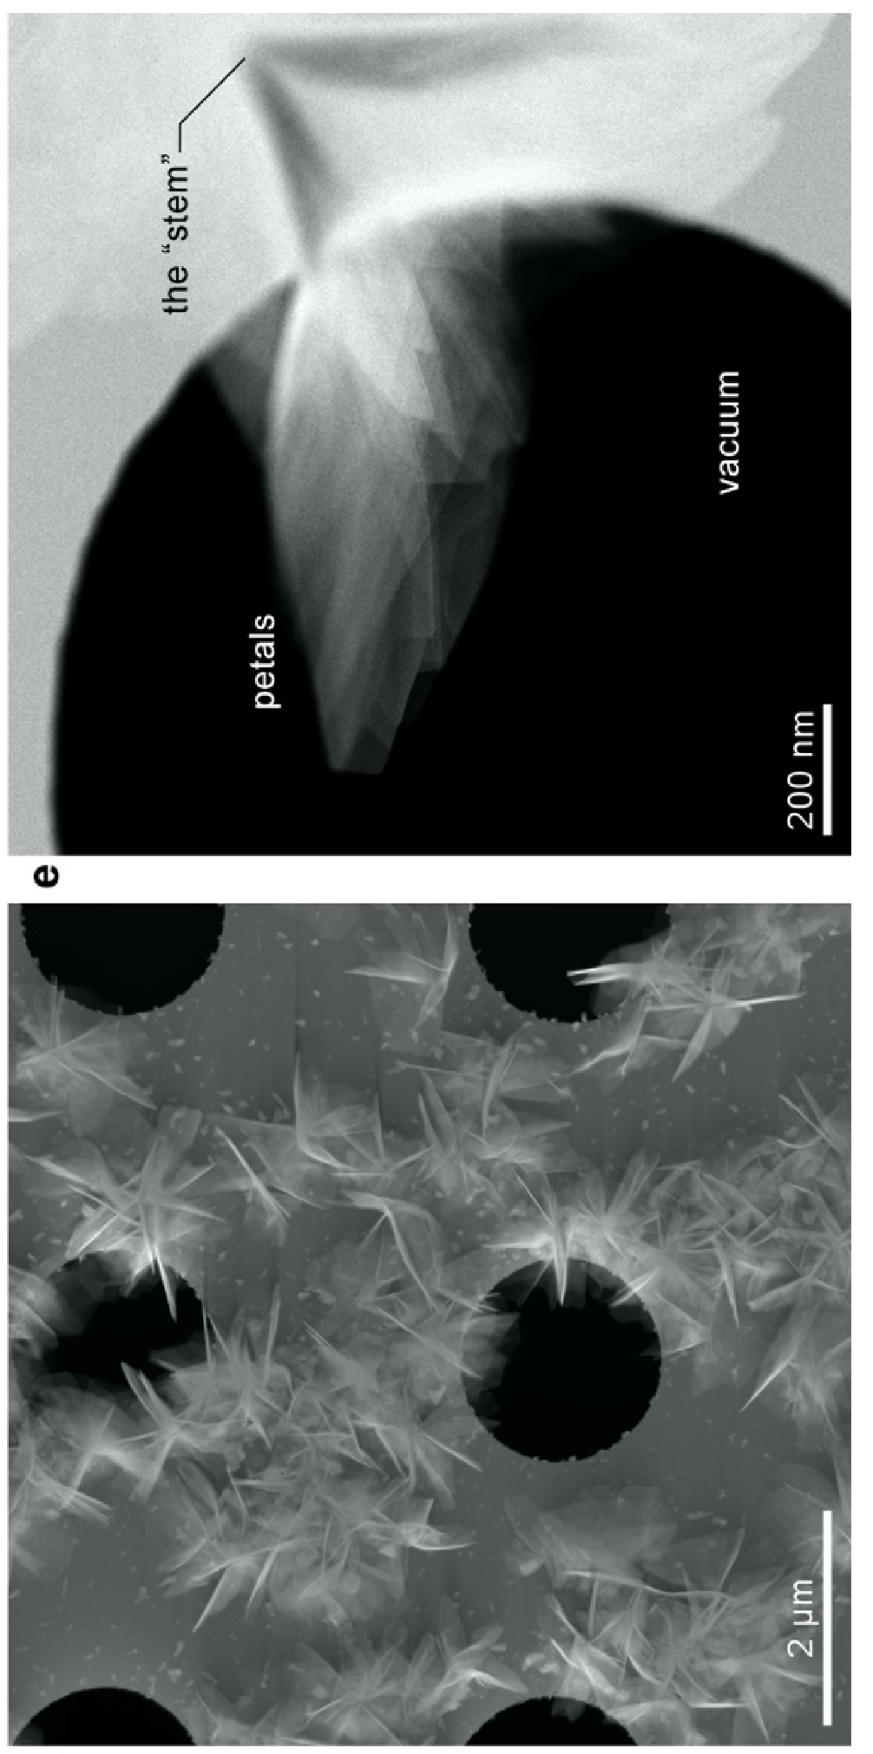
\includegraphics[width=0.49\textwidth,angle=-90]{plots/nanoflowers.pdf}
    \caption{Left: low-magnification TEM image of WS$_2$ nanoflowers
      grown on top of a holey TEM substrate. Right: a magnification of a
      representative {\it petals}
      of a flower and the {\it stem} that connects it to the substrate.
      %
      Note that the black region corresponds to the vacuum (no substrate).
      {\bf needs updating}
      }
    \label{fig:nanoflowers}
\end{figure}
%%%%%%%%%%%%%%%%%%%%%%%%%%%%%%%%%%%%%%%%%%%%%%%%%%%%%%%%%%%%%%%%%%%%%%%%%%%%%%%%%%5

A low-magnification TEM image of the WS$_2$ nanoflowers presented in~\cite{SabryaWS2} is displayed
in the left panel of Fig.~\ref{fig:nanoflowers}.
%
These nanostructures are grown directly in top of a holey TEM substrate.
%
In the right panel of the same figure we show a magnification of a
      representative {\it petals}
      of a specific flower and the {\it stem} that connects it to the substrate.
      %
      Note that the black region corresponds to the vacuum, that is, without
      substrate underneath.
%
These WS$_2$ nanoflowers exhibit a wide variety of thicknesses, orientations
and crystalline structures, therefore representing an ideal laboratory to correlate
structural morphology in WS$_2$ with electronic properties at the nanoscale.
%
Further, these nanoflowers display 3R/2H polytypism,
an important factor that determines the interlayer
interactions within WS$_2$: different stacking types tend to coexist, 
thus complicating the characterization of the physical properties~\cite{Na:2018}.
%
One consequence of the different stacking patterns is the appearance of
spontaneous electrical polarization, leading to modifications on the 
electronic band structure and correspondingly on the band gap~\cite{Lee:2016}.

As mentioned above, one of the most interesting properties of  WS$_2$ is
that when the material
is thinned down to a single monolayer, its indirect band gap of
$E_{\rm BG}\simeq 1.4$ eV
switches to a direct band gap of approximately $E_{\rm BG}\simeq 2.1$ eV.
%
In general, it has been found that the type and magnitude of the bandgap
of WS$_2$ depends quite sensitively on the crystalline structure and
the number of layers that constitute the material.
%
In Table~\ref{table:bgvalues} we collect
representative results for the determination of the bandgap energy $E_{\rm BG}$
and its type in WS$_2$, obtained by means of different experimental and theoretical techniques.
%
 For each reference we indicate separately the bulk results and those
obtained at the monolayer (ML) level.
%
We note that at the monolayer level there is a fair spread of results in the
value of $E_{\rm BG}$, reflecting the challenges of its accurate determination.
 
%%%%%%%%%%%%%%%%%%%%%%%%%%%%%%%%%%%%%%%%%%%%%%%%%%%%%%%%%%%%%%%%%%%%%%%%%%%%%%%%%%%%%
\begin{table}[t]
  \small
  \begin{centering}
   \renewcommand{\arraystretch}{1.20}
\begin{tabular}{ccccc}
\br
Reference                       & Thickness & $E_{\rm BG}$ (eV)  & Band gap type  & Technique \\
\mr
{\cite{Braga:2012}} & bulk   & $1.4\pm0.07$            & indirect  & {Gate-voltage dependence}  \\
\mr
\multirow{2}{*}{\cite{Jo:2014}}                 & ML   & $2.14 $         & direct  & \multirow{2}{*}{Gate-voltage dependence}        \\
& bulk & $1.40 $    & indirect              \\
\mr

\multirow{2}{*}{\cite{Gusakova:2007}} & ML   & $2.03\pm0.03$            & direct  & \multirow{2}{*}{DFT}  \\
& bulk & $1.32\pm0.03 $            & indirect     \\
\mr
\multirow{2}{*}{\cite{Kam:1982}}                  & ML   & $1.76\pm0.03 $      & direct    & \multirow{2}{*}{Absorption edge coefficient fitting}         \\
& bulk & $1.35 $          & indirect        \\
\mr
\cite{Shi:2013}                & ML   & $2.21\pm0.3 $         & direct  & Bethe-Salpeter equation (BSE)        \\                 \br                                         
\end{tabular}
\vspace{0.27cm}
\caption{Representative results for the determination of the bandgap energy $E_{\rm BG}$
  and its type in WS$_2$, obtained by means of different experimental and theoretical techniques.
  %
  For each reference we indicate separately the bulk results and those
  obtained at the monolayer (ML) level.}
    \label{table:bgvalues}
    \end{centering}
\end{table}
%%%%%%%%%%%%%%%%%%%%%%%%%%%%%%%%%%%%%%%%%%%%%%%%%%%%%%%%%%%%%%%%%%%%%%%%%%%%%%%%%%%%%%
